% Provenance (never printed): cycle 3 / 6e "La planete Terre, l'environnement
% et l'action humaine" (the Earth in the Solar System; conditions for life);
% see sources/book1/PROVENANCE.md. Book 1, grade 6, chapter 1.
\chapter{A Terra, um planeta do Sistema Solar}\label{ch:g6:earth-a-planet}

Três sondas robóticas foram mandadas para o espaço. Uma de cada vez, elas
mandam para casa uma imagem, como um cartão-postal. A primeira vem de
Vênus: uma bola pálida envolta em \omterm{def:g4:clouds-rain-snow:cloud}{nuvens} espessas, onde faz calor
suficiente para derreter chumbo e o ar pressiona o chão com um peso
esmagador. A segunda vem de Marte: um \omterm{def:g5:weather-and-climate:desert}{deserto} vermelho, frio e poeirento,
embaixo de um céu ralo. A terceira sonda virou a sua câmera de volta para
casa: uma bola azul e branca, com \omterm{def:g2:water-on-earth:ocean}{oceanos}, \omterm{def:g4:clouds-rain-snow:cloud}{nuvens} e gelo. Três planetas,
vizinhos em volta do mesmo Sol. Por que só um deles é azul?
% ledger: nasa:venus-clouds, nasa:mars-water

\begin{omfigure}
\begin{minipage}[t]{0.31\linewidth}\centering
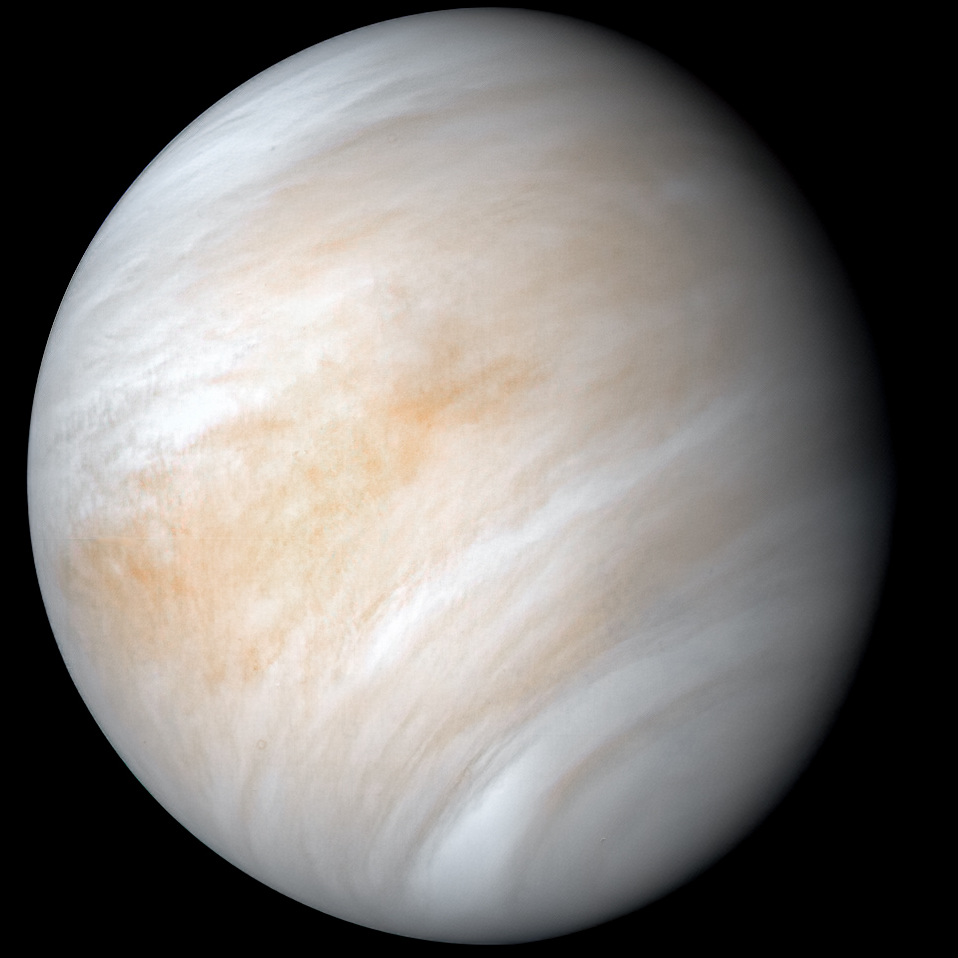
\includegraphics[width=\linewidth]{images/book1/g6-venus-mariner10.jpg}\\[2pt]
{\small Vênus}
\end{minipage}\hfill
\begin{minipage}[t]{0.31\linewidth}\centering
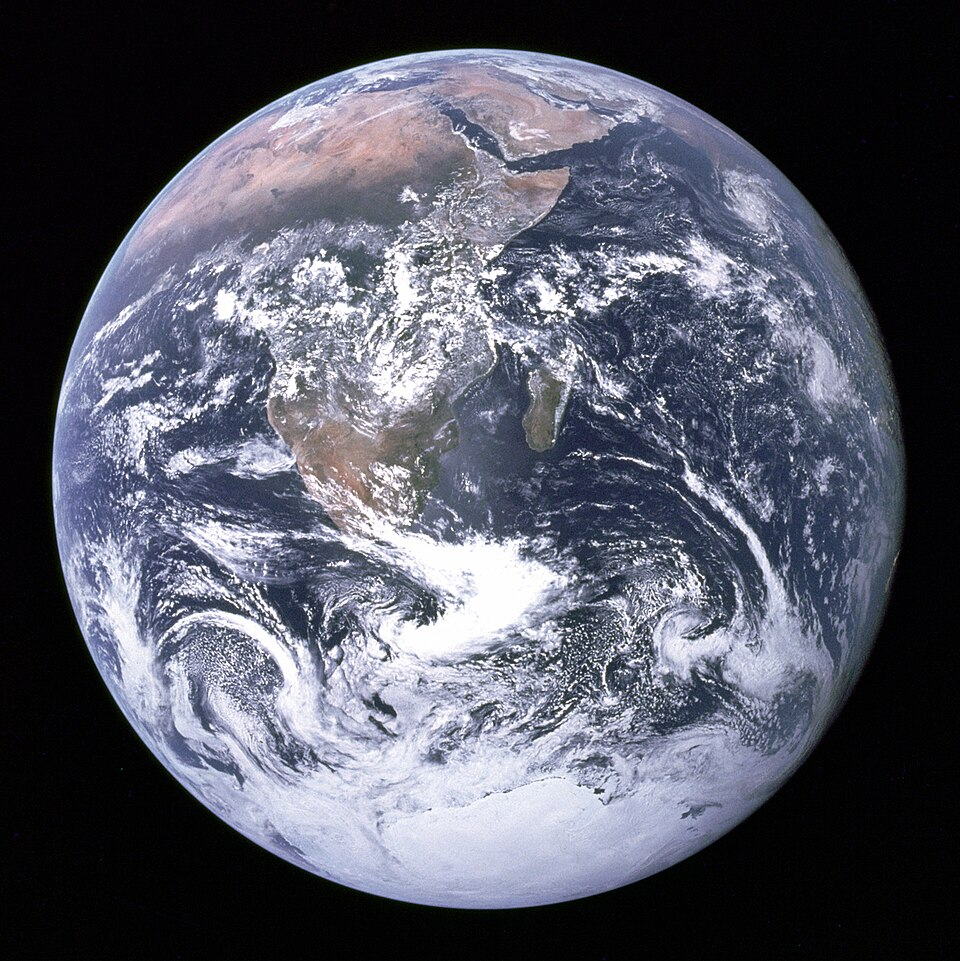
\includegraphics[width=\linewidth]{images/book1/g6-earth-apollo17.jpg}\\[2pt]
{\small A Terra}
\end{minipage}\hfill
\begin{minipage}[t]{0.31\linewidth}\centering
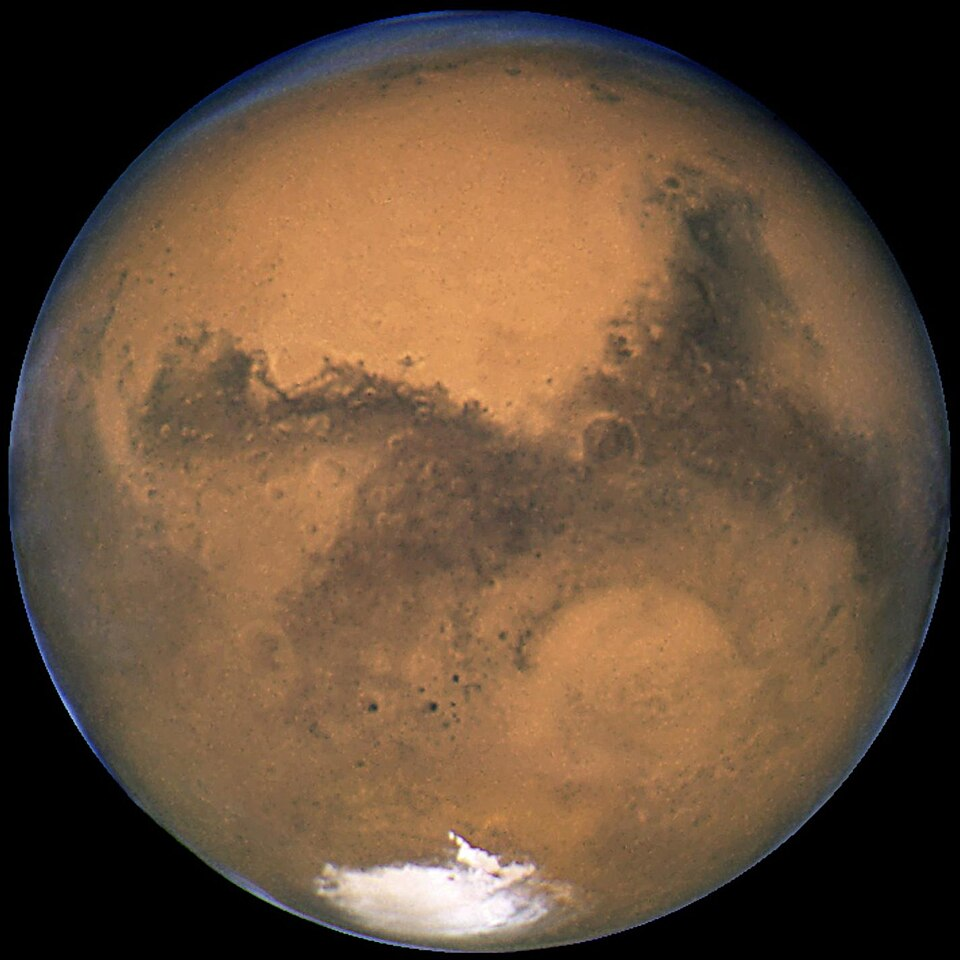
\includegraphics[width=\linewidth]{images/book1/g6-mars-hubble.jpg}\\[2pt]
{\small Marte}
\end{minipage}

\medskip
{\small Três cartões-postais do espaço. Vênus, fotografado pela sonda
Mariner~10 em 1974: vemos só o topo das suas \omterm{def:g4:clouds-rain-snow:cloud}{nuvens}. A Terra, fotografada
pela tripulação da Apollo~17 a caminho da Lua, em 1972: a África, a Arábia
e o gelo da Antártida embaixo de \omterm{def:g4:clouds-rain-snow:cloud}{nuvens} brancas. Marte, fotografado pelo
Telescópio Espacial Hubble em 2003, com uma calota branca de gelo no seu
\omterm{def:g3:continents-and-oceans:poles}{polo}. (Fotos: NASA/JPL-Caltech; NASA; NASA, ESA e Hubble Heritage Team.)}
% ledger: nasa:venus-mariner10, nasa:apollo17-earth, hubble:mars-2003
\end{omfigure}

\begin{recall}
Os livros de física mostraram que o Sol é uma estrela, uma bola enorme de
gás quente que brilha sozinha, e que um planeta é um corpo grande e
redondo que gira em volta de uma estrela e não brilha sozinho: nós o vemos
porque ele reflete a luz da sua estrela. O Sol e tudo o que gira em volta
dele formam o Sistema Solar. Cada planeta viaja em volta do Sol ao longo de
um caminho chamado a sua órbita, e gira sobre si mesmo em torno de um
eixo. O ar à nossa volta pressiona tudo o que toca: é a pressão do ar. A
densidade de um material diz quanto pesa um certo volume dele: um
centímetro cúbico de água pesa 1~grama, então a sua densidade é de 1~grama
por centímetro cúbico; um material mais denso que a água afunda nela, e um
material menos denso flutua. Por fim, cerca de sete décimos da superfície
da Terra são cobertos pelo \omterm{def:g2:water-on-earth:ocean}{oceano} (\cref{ch:g2:water-on-earth}).
\end{recall}

\section{Oito planetas em volta do Sol}

Oito planetas viajam em volta do Sol. Em ordem, do mais próximo ao mais
distante, eles são Mercúrio, Vênus, a Terra, Marte, Júpiter, Saturno, Urano
e Netuno. Uma frase pode ajudar a lembrar a ordem: \emph{Minha Vó Tem
Muitas Joias, Só Usa No Natal} (Mercúrio, Vênus, Terra, Marte, Júpiter,
Saturno, Urano, Netuno).

O desenho abaixo mostra os oito planetas lado a lado, desenhados na mesma
escala: se um planeta é duas vezes mais largo que outro, o seu círculo
também é duas vezes mais largo.

\begin{omfigure}
\pgfplotstableread{figdata/out/grade-6-planets-sizes.dat}\gsixsizes
\begin{tikzpicture}
  \draw[black!40] (-0.2,0) -- (13.8,0);
  \pgfplotstablegetrowsof{\gsixsizes}
  \pgfmathtruncatemacro{\gsixlast}{\pgfplotsretval-1}
  \foreach \i in {0,...,\gsixlast}{
    \pgfplotstablegetelem{\i}{x_cm}\of\gsixsizes \let\gx\pgfplotsretval
    \pgfplotstablegetelem{\i}{d_cm}\of\gsixsizes \let\gd\pgfplotsretval
    \pgfplotstablegetelem{\i}{name}\of\gsixsizes \let\gn\pgfplotsretval
    \pgfplotstablegetelem{\i}{d_km}\of\gsixsizes \let\gk\pgfplotsretval
    \pgfmathsetmacro{\gr}{\gd/2}
    \ifnum\i<4
      \fill[brown!70!black, draw=black!60, line width=0.3pt] (\gx,\gr) circle (\gr);
    \else
      \fill[orange!35, draw=black!60, line width=0.3pt] (\gx,\gr) circle (\gr);
    \fi
    \node[font=\scriptsize, rotate=40, anchor=north east, inner sep=1pt]
      at (\gx+0.08,-0.08) {\ifcase\i\relax Mercúrio\or Vênus\or Terra\or Marte\or Júpiter\or Saturno\or Urano\or Netuno\fi};
  }
  \node[font=\scriptsize, align=left, anchor=north west] at (-0.2,4.15)
    {\tikz\fill[brown!70!black, draw=black!60] (0,0) circle (2.2pt); planetas rochosos\\
     \tikz\fill[orange!35, draw=black!60] (0,0) circle (2.2pt); planetas gigantes};
  \draw[|-|, black!70] (0,2.2) -- (1,2.2)
    node[midway, above, font=\scriptsize] {35\,000 km};
\end{tikzpicture}

{\small Os oito planetas desenhados em escala (diâmetros da tabela de dados
planetários da NASA). As distâncias entre eles não estão em escala: elas são
grandes demais para caber em qualquer página.}
% ledger: planet:Mercury.diameter, planet:Venus.diameter, planet:Earth.diameter, planet:Mars.diameter, planet:Jupiter.diameter, planet:Saturn.diameter, planet:Uranus.diameter, planet:Neptune.diameter (figdata/grade-6/planets.py, part sizes)
\end{omfigure}

Os quatro planetas mais próximos do Sol são pequenos. Os quatro seguintes
são gigantes: Júpiter é cerca de 11 vezes mais largo que a Terra. E o Sol?
Desenhado na mesma escala que os planetas acima, ele seria um disco de
cerca de 40~centímetros de largura --- mais largo que esta página.
% ledger: planet:Jupiter.diameter, planet:Earth.diameter, sun:R (planets.py: sun_cm = 39.9 cm)

O tamanho não é a única diferença. A tabela abaixo dá, para cada planeta, o
seu diâmetro, a sua densidade (em gramas por centímetro cúbico) e a sua
distância do Sol.

\begin{center}
\small
\begin{tabular}{lrrrr}
\hline
planeta & diâmetro (km) & densidade (g/cm$^3$) & distância do Sol (milhões de km)\\
\hline
Mercúrio & 4\,879 & 5.4 & 58\\
Vênus & 12\,104 & 5.2 & 108\\
Terra & 12\,756 & 5.5 & 150\\
Marte & 6\,792 & 3.9 & 228\\
\hline
Júpiter & 142\,984 & 1.3 & 779\\
Saturno & 120\,536 & 0.7 & 1\,432\\
Urano & 51\,118 & 1.3 & 2\,867\\
Netuno & 49\,528 & 1.6 & 4\,515\\
\hline
\end{tabular}
% ledger: planet:Mercury.diameter, planet:Venus.diameter, planet:Earth.diameter, planet:Mars.diameter, planet:Jupiter.diameter, planet:Saturn.diameter, planet:Uranus.diameter, planet:Neptune.diameter, planet:Mercury.density, planet:Venus.density, planet:Earth.density, planet:Mars.density, planet:Jupiter.density, planet:Saturn.density, planet:Uranus.density, planet:Neptune.density, planet:Mercury.dist, planet:Venus.dist, planet:Earth.dist, planet:Mars.dist, planet:Jupiter.dist, planet:Saturn.dist, planet:Uranus.dist, planet:Neptune.dist (figdata/grade-6/planets.py, main table)
\end{center}

As densidades dividem os planetas em duas famílias, sem nada no meio: os
quatro primeiros são densos, com mais de 3.9~gramas por centímetro cúbico,
como a \omterm{def:g3:stones-pebbles-sand:rock}{rocha} e o metal; os quatro últimos são leves, com menos de
1.7~grama por centímetro cúbico.

\begin{definition}[Planetas rochosos e planetas gigantes]\label{def:g6:earth-a-planet:planet-types}
Um \emph{planeta rochoso}\index{planeta rochoso} é um planeta pequeno e
denso, feito de \omterm{def:g3:stones-pebbles-sand:rock}{rocha} e de metal, com uma superfície sólida onde uma sonda
pode pousar: Mercúrio, Vênus, a Terra e Marte. Um \emph{planeta
gigante}\index{planeta gigante} é um planeta muito grande e de baixa densidade,
feito sobretudo de gases e de líquidos, sem uma superfície sólida onde
pousar: Júpiter, Saturno, Urano e Netuno.
% ledger: nasa:planet-families
\end{definition}

\begin{omfigure}
\begin{minipage}[c]{0.6\linewidth}\centering
\begin{tikzpicture}
  \begin{axis}[ybar, bar width=11pt, width=\linewidth, height=5.4cm,
      ymin=0, ymax=6.2, xmin=-0.6, xmax=7.6,
      xtick={0,...,7}, xticklabels={Mercúrio,Vênus,Terra,Marte,Júpiter,Saturno,Urano,Netuno},
      xticklabel style={rotate=40, anchor=north east, font=\scriptsize},
      ytick={0,1,...,6}, ylabel={densidade (g/cm$^3$)},
      tick label style={font=\scriptsize}, label style={font=\scriptsize},
      axis x line*=bottom, axis y line*=left]
    \addplot[fill=brown!70!black, draw=black!60, bar shift=0pt, restrict x to domain=0:3]
      table[x=idx, y=density_gcm3] {figdata/out/grade-6-planets-density.dat};
    \addplot[fill=orange!35, draw=black!60, bar shift=0pt, restrict x to domain=4:7]
      table[x=idx, y=density_gcm3] {figdata/out/grade-6-planets-density.dat};
    \draw[blue!60!black, densely dashed] (axis cs:-0.6,1) -- (axis cs:7.6,1);
    \node[font=\scriptsize, blue!60!black, anchor=south, inner sep=1pt]
      at (axis cs:5,1) {água};
  \end{axis}
\end{tikzpicture}
\end{minipage}\hfill
\begin{minipage}[c]{0.36\linewidth}\centering
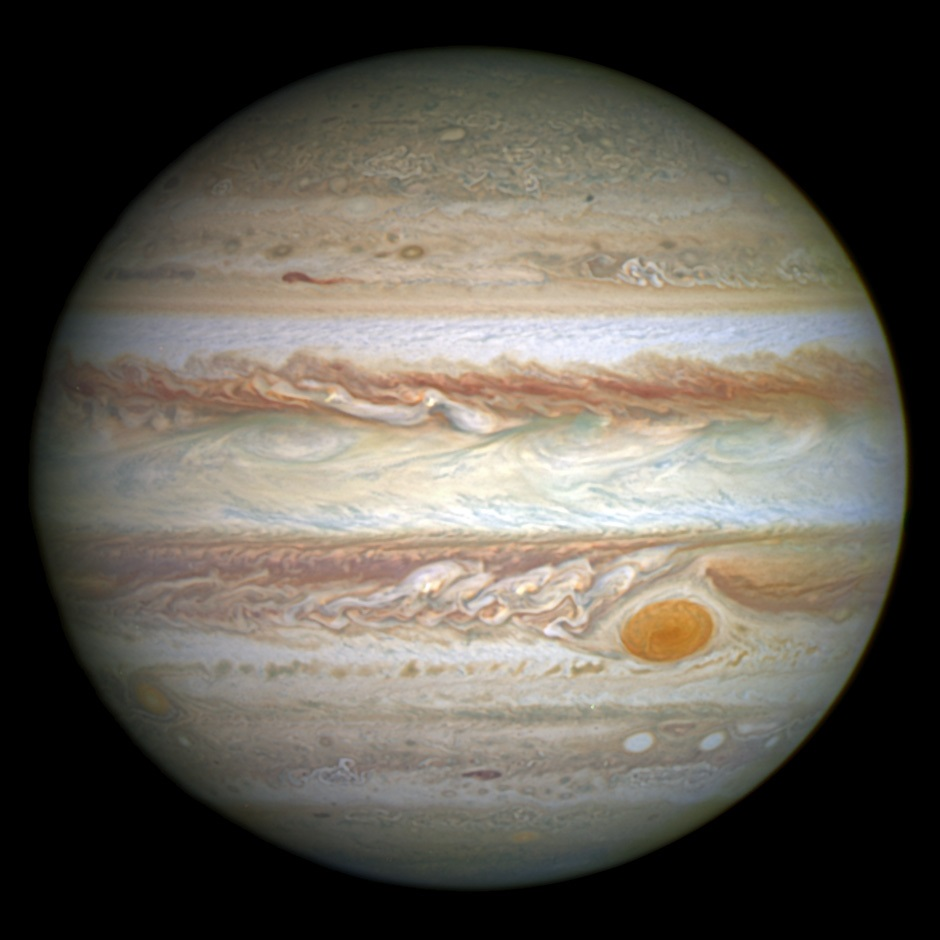
\includegraphics[width=0.9\linewidth]{images/book1/g6-jupiter-hubble.jpg}\\[2pt]
{\small Júpiter, fotografado pelo Telescópio Espacial Hubble em 2014.
(Foto: NASA, ESA, A.~Simon.)}
% ledger: hubble:jupiter-2014
\end{minipage}

\smallskip
{\small À esquerda: a densidade dos oito planetas; a linha tracejada é a
densidade da água. À direita: o que vemos de um \omterm{def:g6:earth-a-planet:planet-types}{planeta gigante} é o topo
das suas \omterm{def:g4:clouds-rain-snow:cloud}{nuvens}.}
% ledger: planet:Mercury.density, planet:Venus.density, planet:Earth.density, planet:Mars.density, planet:Jupiter.density, planet:Saturn.density, planet:Uranus.density, planet:Neptune.density (figdata/grade-6/planets.py, part density)
\end{omfigure}

A fotografia de Júpiter mostra faixas de \omterm{def:g4:clouds-rain-snow:cloud}{nuvens}, claras e escuras, e um
oval vermelho: a Grande Mancha Vermelha, uma \omterm{def:g5:natural-hazards:storm}{tempestade} gigante maior que a
Terra inteira, que sopra há centenas de anos. Embaixo das \omterm{def:g4:clouds-rain-snow:cloud}{nuvens} não há
chão: só gases, sobretudo hidrogênio e hélio, que ficam cada vez mais
densos quanto mais fundo se vai.
% ledger: nasa:jupiter-gas

\begin{remark}[Um planeta mais leve que a água]\label{rem:g6:earth-a-planet:saturn}
Saturno é o único planeta cuja densidade é menor que a da água: cerca de
0.7~grama por centímetro cúbico. Se existisse uma banheira grande o
bastante para contê-lo, Saturno flutuaria!
% ledger: nasa:saturn-float, planet:Saturn.density
\end{remark}

\section{A que distância ficam os planetas uns dos outros?}

Os planetas não são só muito diferentes no tamanho; eles também ficam muito
longe uns dos outros. A Terra fica a cerca de 150~milhões de quilômetros do
Sol. Netuno, o planeta mais distante, fica 30~vezes mais longe: cerca de
4500~milhões de quilômetros. O desenho abaixo coloca os oito planetas numa
só linha, às suas distâncias do Sol, em escala.
% ledger: planet:Earth.dist, planet:Neptune.dist

\begin{omfigure}
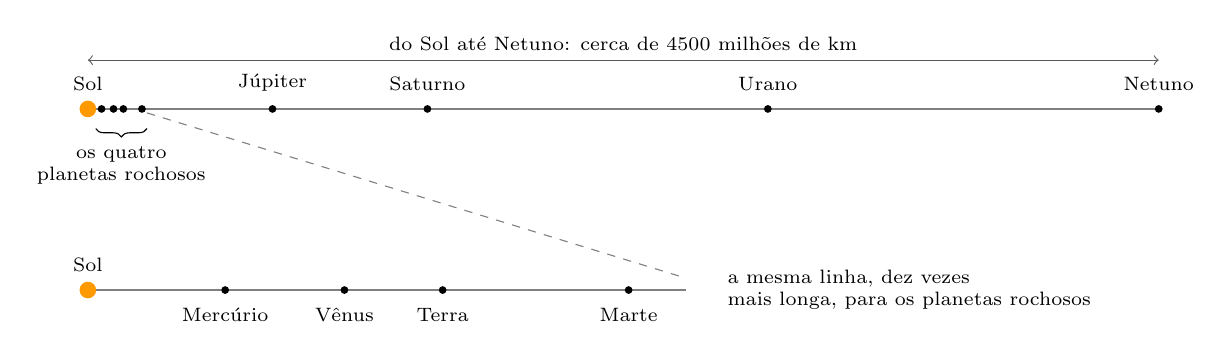
\begin{tikzpicture}
  % whole system
  \draw[thick, gray] (0,0) -- (13.6,0);
  \fill[orange!80!yellow] (0,0) circle (3pt);
  \node[font=\scriptsize, above=3pt] at (0,0) {Sol};
  \foreach \n/\x/\lab in {Mercúrio/0.174/, Vênus/0.326/, Terra/0.451/, Marte/0.687/,
                          Júpiter/2.345/Júpiter, Saturno/4.313/Saturno, Urano/8.636/Urano, Netuno/13.6/Netuno} {
    \fill (\x,0) circle (1.4pt);
    \node[font=\scriptsize, above=3pt] at (\x,0) {\lab};
  }
  \draw[decorate, decoration={brace, amplitude=3pt, mirror}] (0.1,-0.25) -- (0.75,-0.25)
    node[midway, below=3pt, font=\scriptsize, align=center] {os quatro\\ planetas rochosos};
  \draw[<->, thin, gray!70!black] (0,0.62) -- (13.6,0.62) node[midway, above, font=\scriptsize, black] {do Sol até Netuno: cerca de 4500 milhões de km};
  % the inner system, ten times larger
  \begin{scope}[yshift=-2.3cm]
    \draw[thick, gray] (0,0) -- (7.6,0);
    \fill[orange!80!yellow] (0,0) circle (3pt);
    \node[font=\scriptsize, above=3pt] at (0,0) {Sol};
    \foreach \n/\x in {Mercúrio/1.744, Vênus/3.259, Terra/4.506, Marte/6.868} {
      \fill (\x,0) circle (1.4pt);
      \node[font=\scriptsize, below=3pt] at (\x,0) {\n};
    }
    \node[font=\scriptsize, anchor=west, align=left] at (8.0,0) {a mesma linha, dez vezes\\ mais longa, para os planetas rochosos};
  \end{scope}
  \draw[dashed, gray] (0.75,-0.05) -- (7.6,-2.15);
\end{tikzpicture}

{\small As distâncias dos planetas ao Sol, em escala. Em cima: o Sistema
Solar inteiro, do Sol até Netuno. Embaixo: os quatro \omterm{def:g6:earth-a-planet:planet-types}{planetas rochosos},
ampliados dez vezes. Os tamanhos dos pontos não estão em escala.}
% ledger: planet:Mercury.dist, planet:Venus.dist, planet:Earth.dist, planet:Mars.dist, planet:Jupiter.dist, planet:Saturn.dist, planet:Uranus.dist, planet:Neptune.dist (figdata/grade-6/planets.py, part dist)
\end{omfigure}

Os quatro \omterm{def:g6:earth-a-planet:planet-types}{planetas rochosos} ficam todos perto do Sol; os quatro \omterm{def:g6:earth-a-planet:planet-types}{planetas
gigantes} ficam bem longe, com distâncias enormes entre eles. Só a distância entre Marte e Júpiter, cerca de 550~milhões de quilômetros, é mais que o dobro da distância do Sol até Marte.
% ledger: planet:Mars.dist, planet:Jupiter.dist

É difícil desenhar os tamanhos e as distâncias na mesma escala: os planetas
viram pontinhos invisíveis. Um \emph{modelo em escala} ajuda a imaginar as
duas coisas ao mesmo tempo.

\begin{method}[Construir um modelo em escala do Sistema Solar]\label{met:g6:earth-a-planet:scale-model}
\begin{enumerate}
  \item Escolha o tamanho da Terra no modelo, por exemplo 1~cm.
  \item Descubra quantos quilômetros reais 1~cm do modelo representa:
        divida o diâmetro real da Terra (12\,756~km) pelo seu tamanho no
        modelo.
  \item Divida cada tamanho real e cada distância real por esse número.
        Depois mude as unidades para algo fácil de imaginar (centímetros,
        metros, quilômetros).
\end{enumerate}
% ledger: planet:Earth.diameter
\end{method}

\begin{example}[Uma bolinha de gude no lugar da Terra]\label{ex:g6:earth-a-planet:marble}
Se a Terra é uma bolinha de gude de 1~cm de largura, 1~cm representa
12\,756~km. O Sol, com 1\,391\,400~km de largura, vira uma bola de $1\,391\,400 \div 12\,756 \approx
109$~cm de largura: uma bola mais alta que uma criança pequena. A Terra fica a 150~milhões~de~km do Sol:
$149\,600\,000 \div 12\,756 \approx 11\,700$~cm, ou seja, cerca de
117~metros, o comprimento de um campo de futebol.
% ledger: planet:Earth.diameter, sun:R, planet:Earth.dist
\end{example}

\begin{center}\small
\begin{tabular}{|l|c|c|}
\hline
\textbf{corpo} & \textbf{tamanho no modelo (cm)} & \textbf{distância do Sol (m)} \\
\hline
o Sol & 109 & --- \\
Mercúrio & 0.38 & 45 \\
Vênus & 0.95 & 85 \\
a Terra & 1.00 & 117 \\
Marte & 0.53 & 179 \\
Júpiter & 11.21 & 610 \\
Saturno & 9.45 & 1123 \\
Urano & 4.01 & 2248 \\
Netuno & 3.88 & 3540 \\
\hline
\end{tabular}
\end{center}
% ledger: sun:R, planet:Mercury.diameter, planet:Venus.diameter, planet:Earth.diameter, planet:Mars.diameter, planet:Jupiter.diameter, planet:Saturn.diameter, planet:Uranus.diameter, planet:Neptune.diameter, planet:Mercury.dist, planet:Venus.dist, planet:Earth.dist, planet:Mars.dist, planet:Jupiter.dist, planet:Saturn.dist, planet:Uranus.dist, planet:Neptune.dist (figdata/grade-6/planets.py, part model)

Nesse modelo, o Sistema Solar inteiro, até Netuno, se espalha por um
círculo de 7~km de largura, com uma bola grande no meio e oito bolinhas e
bolas, a maior do tamanho de uma toranja, espalhadas por ele. O Sistema
Solar é feito sobretudo de espaço vazio.

\section{Vênus, a Terra e Marte}

Vênus, a Terra e Marte são vizinhos, e os três são \omterm{def:g6:earth-a-planet:planet-types}{planetas rochosos}. Vênus
tem quase o mesmo tamanho que a Terra: o seu diâmetro é 95~\% do da Terra.
Marte é menor: o seu diâmetro é cerca da metade do da Terra. Mesmo assim,
esses três planetas não poderiam ser mais diferentes.
% ledger: planet:Venus.diameter, planet:Earth.diameter, planet:Mars.diameter (planets.py: 94.9 %)

\paragraph{Vênus.} Vênus é envolto numa camada espessa de ar, feito
sobretudo de gás carbônico, com \omterm{def:g4:clouds-rain-snow:cloud}{nuvens} densas de ácido sulfúrico, um ácido
que queima. O seu ar é tão espesso que pressiona o chão com uma força
92~vezes maior que a do ar da Terra sobre o nosso. Na superfície, a
temperatura é de cerca de 464~$^\circ$C: calor suficiente para derreter
chumbo. Nenhuma água consegue ficar líquida ali.
% ledger: nasa:venus-clouds, planet:Venus.psurf, planet:Venus.Tmean

\paragraph{Marte.} Marte é um \omterm{def:g5:weather-and-climate:desert}{deserto} frio, seco e poeirento. O seu ar
também é feito sobretudo de gás carbônico, mas é muito ralo: ele pressiona
o chão cerca de cem vezes menos que o ar da Terra. A temperatura média é de
$-65$~$^\circ$C. Hoje há água ali, mas congelada: como gelo nas calotas
polares e embaixo do chão perto dos \omterm{def:g3:continents-and-oceans:poles}{polos}. Mas Marte nem sempre foi assim:
há bilhões de anos, \omterm{def:g1:landscapes-around-us:water}{rios} corriam em Marte, \omterm{def:g1:landscapes-around-us:water}{lagos} se formavam e \omterm{def:g5:water-shapes-the-land:flood}{inundações} o
atravessavam.
% ledger: nasa:mars-water, planet:Mars.psurf, planet:Mars.Tmean

\paragraph{A Terra.} Entre os dois, a Terra tem um ar que pressiona o chão
com cerca de 1~bar (a unidade usada para comparar a pressão do ar nos
planetas), uma temperatura média de 15~$^\circ$C e \omterm{def:g2:water-on-earth:ocean}{oceanos} de água
líquida.
% ledger: planet:Earth.psurf, planet:Earth.Tmean

\begin{omfigure}
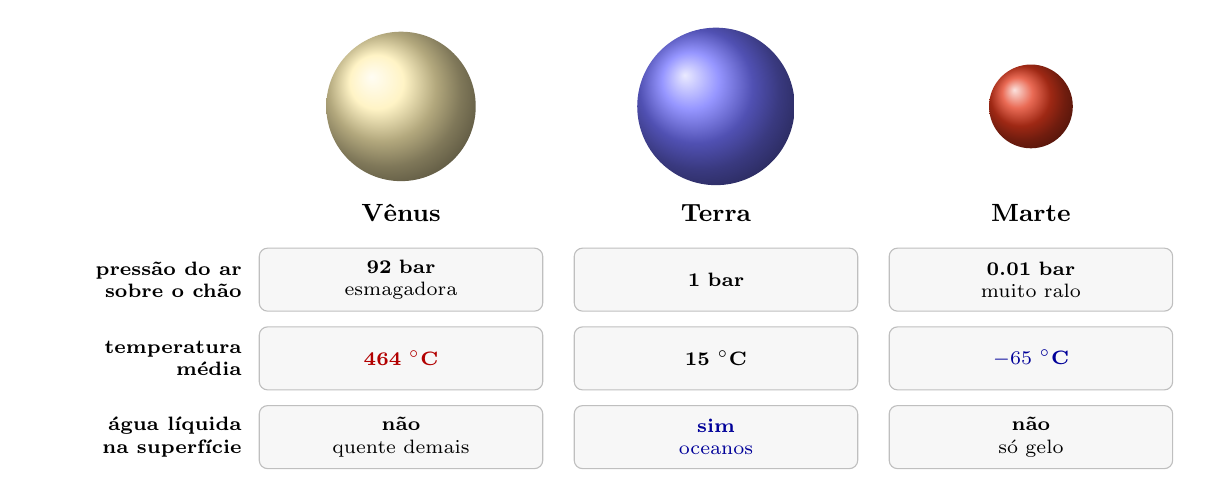
\begin{tikzpicture}[x=1cm, y=1cm,
    lab/.style={font=\scriptsize, align=center, text width=3.6cm},
    row/.style={font=\scriptsize\bfseries, anchor=east, align=right, text width=2.6cm}]
  % discs to scale: diameters 94.9 %, 100 %, 53.2 % of the Earth's (planets.py)
  \shade[ball color=yellow!60!orange!30] (3,0) circle (0.949);
  \shade[ball color=blue!55] (7,0) circle (1.0);
  \shade[ball color=red!55!brown] (11,0) circle (0.532);
  \node[font=\small\bfseries] at (3,-1.35) {Vênus};
  \node[font=\small\bfseries] at (7,-1.35) {Terra};
  \node[font=\small\bfseries] at (11,-1.35) {Marte};
  \foreach \y/\t in {-2.2/{pressão do ar\\sobre o chão}, -3.2/{temperatura\\média},
                     -4.2/{água líquida\\na superfície}}
    {\node[row] at (1.1,\y) {\t};}
  \foreach \x in {3,7,11}{
    \foreach \y in {-2.2,-3.2,-4.2}{
      \draw[rounded corners=3pt, black!25, fill=black!3] (\x-1.8,\y-0.4) rectangle (\x+1.8,\y+0.4);}}
  \node[lab] at (3,-2.2) {\textbf{92 bar}\\esmagadora};
  \node[lab] at (7,-2.2) {\textbf{1 bar}};
  \node[lab] at (11,-2.2) {\textbf{0.01 bar}\\muito ralo};
  \node[lab, text=red!70!black] at (3,-3.2) {\textbf{464~$^\circ$C}};
  \node[lab] at (7,-3.2) {\textbf{15~$^\circ$C}};
  \node[lab, text=blue!60!black] at (11,-3.2) {\textbf{$-65$~$^\circ$C}};
  \node[lab] at (3,-4.2) {\textbf{não}\\quente demais};
  \node[lab, text=blue!60!black] at (7,-4.2) {\textbf{sim}\\oceanos};
  \node[lab] at (11,-4.2) {\textbf{não}\\só gelo};
\end{tikzpicture}

{\small Vênus, a Terra e Marte comparados. Os três discos estão desenhados
em escala. (Valores: tabela de dados planetários da NASA.)}
% ledger: planet:Venus.psurf, planet:Earth.psurf, planet:Mars.psurf, planet:Mercury.Tmean, planet:Venus.Tmean, planet:Earth.Tmean, planet:Mars.Tmean, planet:Jupiter.Tmean, planet:Saturn.Tmean, planet:Uranus.Tmean, planet:Neptune.Tmean, nasa:mars-water
\end{omfigure}

\paragraph{Calor e frio.} Perto do Sol, um planeta recebe muito da sua luz
e do seu calor; longe dele, muito pouco. Então, quanto mais longe do Sol
fica um planeta, mais frio ele deveria ser. O gráfico abaixo mostra que
isso é verdade da Terra para fora: os \omterm{def:g6:earth-a-planet:planet-types}{planetas gigantes}, lá longe, são
mundos gelados. Mas olhe para Vênus: ele fica quase duas vezes mais longe
do Sol que Mercúrio, e mesmo assim é mais quente! O seu ar espesso de gás
carbônico prende o calor do Sol como um cobertor pesado e não o deixa
escapar. Mercúrio, quase sem ar, não consegue guardar o seu calor.
% ledger: planet:Mercury.Tmean, planet:Venus.Tmean, planet:Earth.Tmean, planet:Mars.Tmean, planet:Jupiter.Tmean, planet:Saturn.Tmean, planet:Uranus.Tmean, planet:Neptune.Tmean, planet:Mercury.dist, planet:Venus.dist, planet:Earth.dist, planet:Mars.dist, planet:Jupiter.dist, planet:Saturn.dist, planet:Uranus.dist, planet:Neptune.dist, nasa:venus-clouds, planet:Mercury.psurf

\begin{omfigure}
\begin{tikzpicture}
  \begin{axis}[ybar, bar width=14pt, width=0.86\linewidth, height=6cm,
      ymin=-270, ymax=520, xmin=-0.6, xmax=7.6,
      xtick={0,...,7},
      xticklabels={{Mercúrio\\58}, {Vênus\\108}, {Terra\\150}, {Marte\\228},
                   {Júpiter\\779}, {Saturno\\1432}, {Urano\\2867}, {Netuno\\4515}},
      xticklabel style={align=center, font=\scriptsize},
      axis x line*=bottom, axis y line*=left,
      xticklabel pos=lower, ytick={-200,-100,...,500},
      ylabel={temperatura média ($^\circ$C)}, xlabel={planeta e distância do Sol (milhões de km)},
      tick label style={font=\scriptsize}, label style={font=\scriptsize},
      nodes near coords, nodes near coords style={font=\tiny},
      every node near coord/.append style={/pgf/number format/1000 sep={}}]
    \addplot[fill=orange!50, draw=black!60, bar shift=0pt]
      table[x=idx, y=tmean_C] {figdata/out/grade-6-planets-temp.dat};
    \draw[black!50] (axis cs:-0.6,0) -- (axis cs:7.6,0);
  \end{axis}
\end{tikzpicture}

{\small A temperatura média dos planetas, em ordem de distância do Sol.
Vênus quebra a regra: ele é mais quente que Mercúrio, que fica mais perto
do Sol. (Valores: tabela de dados planetários da NASA.)}
% ledger: planet:Mercury.Tmean, planet:Venus.Tmean, planet:Earth.Tmean, planet:Mars.Tmean, planet:Jupiter.Tmean, planet:Saturn.Tmean, planet:Uranus.Tmean, planet:Neptune.Tmean, planet:Mercury.dist, planet:Venus.dist, planet:Earth.dist, planet:Mars.dist, planet:Jupiter.dist, planet:Saturn.dist, planet:Uranus.dist, planet:Neptune.dist (figdata/grade-6/planets.py, part temp)
\end{omfigure}

\section{O que torna a vida possível na Terra}

A Terra é o único planeta onde sabemos que existe vida. Os seres vivos
precisam de várias condições ao mesmo tempo, e a Terra tem todas elas.

\begin{itemize}
  \item \textbf{Água líquida.} Todos os seres vivos precisam de água
        líquida: a Terra tem \omterm{def:g2:water-on-earth:ocean}{oceanos}, \omterm{def:g1:landscapes-around-us:water}{rios} e \omterm{def:g1:landscapes-around-us:water}{lagos}.
  \item \textbf{Temperaturas amenas.} Na superfície da Terra, a água
        congela a 0~$^\circ$C e ferve a 100~$^\circ$C (física). Com uma
        média de 15~$^\circ$C, as temperaturas da Terra ficam quase sempre
        entre as duas, então a sua água continua líquida.
  \item \textbf{A distância certa do Sol.} Mais perto do Sol, como Vênus,
        um planeta corre o risco de ficar quente demais; mais longe, como
        Marte, frio demais. A Terra fica na distância certa para ter água
        líquida.
  \item \textbf{Uma atmosfera.} A camada de ar em volta da Terra mantém a
        sua superfície aquecida à noite, dá aos seres vivos os gases de que
        eles precisam, e pressiona os \omterm{def:g2:water-on-earth:ocean}{oceanos} o bastante para que a sua água
        continue líquida. Em Marte, o ar é tão ralo que a água líquida não
        consegue durar muito na superfície: ela congela ou vira vapor.
\end{itemize}
% ledger: nasa:mars-water, planet:Earth.Tmean

\begin{remark}[Houve vida em Marte?]\label{rem:g6:earth-a-planet:mars-life}
Como Marte já teve \omterm{def:g1:landscapes-around-us:water}{rios} e \omterm{def:g1:landscapes-around-us:water}{lagos}, os cientistas se perguntam se seres vivos
minúsculos poderiam ter vivido ali, há muito tempo, quando Marte era mais
quente e úmido. Os cientistas não esperam encontrar seres vivos em Marte
hoje; com jipes robóticos, eles procuram nas suas \omterm{def:g3:stones-pebbles-sand:rock}{rochas} sinais de uma
vida que existiu há muito tempo.
% ledger: nasa:mars-water
\end{remark}

\section{A Terra vista do espaço}

Durante milhares de anos, as pessoas só podiam imaginar como era o seu
planeta visto de fora. Em 24~de~dezembro~de~1968, os astronautas da
Apollo~8, em órbita em volta da Lua, viram a Terra nascer acima do
horizonte cinzento da Lua, e um deles, Bill Anders, tirou a fotografia
abaixo.
% ledger: nasa:earthrise

\begin{omfigure}
\begin{minipage}[c]{0.46\linewidth}\centering
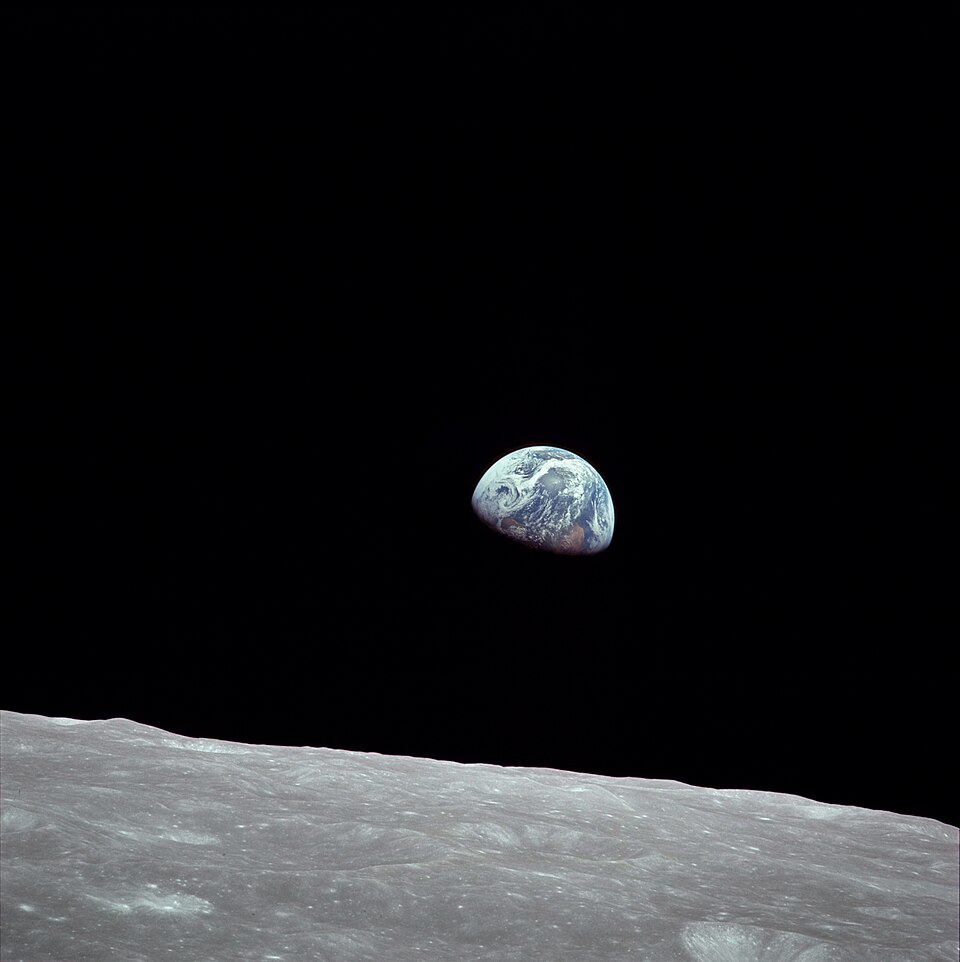
\includegraphics[width=0.85\linewidth]{images/book1/g6-earthrise.jpg}
\end{minipage}\hfill
\begin{minipage}[c]{0.5\linewidth}
{\small \emph{Earthrise} (``o nascer da Terra''): a Terra acima do
horizonte da Lua, fotografada da Apollo~8 em órbita em volta da Lua, em
24~de~dezembro~de~1968. (Foto: NASA, Bill Anders.)}

\medskip
{\small Observe as cores: o azul dos \omterm{def:g2:water-on-earth:ocean}{oceanos}, os redemoinhos brancos das
\omterm{def:g4:clouds-rain-snow:cloud}{nuvens}, o marrom da terra. Em toda a volta, o preto do espaço; em primeiro
plano, o chão cinzento e morto da Lua, sem água e sem ar.}
\end{minipage}
% ledger: nasa:earthrise
\end{omfigure}

Vista do espaço, a Terra é sobretudo azul: o \omterm{def:g2:water-on-earth:ocean}{oceano} cobre cerca de sete
décimos da sua superfície. \omterm{def:g4:clouds-rain-snow:cloud}{Nuvens} brancas de gotículas de água giram acima
dele, e gelo branco cobre os \omterm{def:g3:continents-and-oceans:poles}{polos}. Os \omterm{def:g3:continents-and-oceans:continent}{continentes} são marrons onde são
secos, e verdes onde as plantas crescem. O próprio ar não pode ser visto, mas as \omterm{def:g4:clouds-rain-snow:cloud}{nuvens}
que flutuam nele mostram que ele está ali. De todos os planetas do Sistema
Solar, só a Terra mostra essas cores juntas: água líquida, \omterm{def:g4:clouds-rain-snow:cloud}{nuvens} e plantas
vivas.
% ledger: wss:ocean-cover, nasa:apollo17-earth

\begin{history}[O pálido ponto azul]
\begin{minipage}[c]{0.66\linewidth}
Em 14~de~fevereiro~de~1990, a sonda espacial Voyager~1 estava a cerca de
6~bilhões de quilômetros do Sol, mais longe que Netuno. Antes de deixar o
Sistema Solar para trás, ela virou a sua câmera de volta e tirou uma foto
da Terra. Na fotografia, o nosso planeta é um único pontinho brilhante,
menor que um grão de poeira, preso num raio de luz do Sol. O astrônomo Carl
Sagan escreveu sobre ela: ``Olhe de novo para esse ponto. É aqui. É a nossa
casa. Somos nós.''
% ledger: nasa:pale-blue-dot
\end{minipage}\hfill
\begin{minipage}[c]{0.3\linewidth}\centering
\begin{tikzpicture}
  \node[inner sep=0] (img) {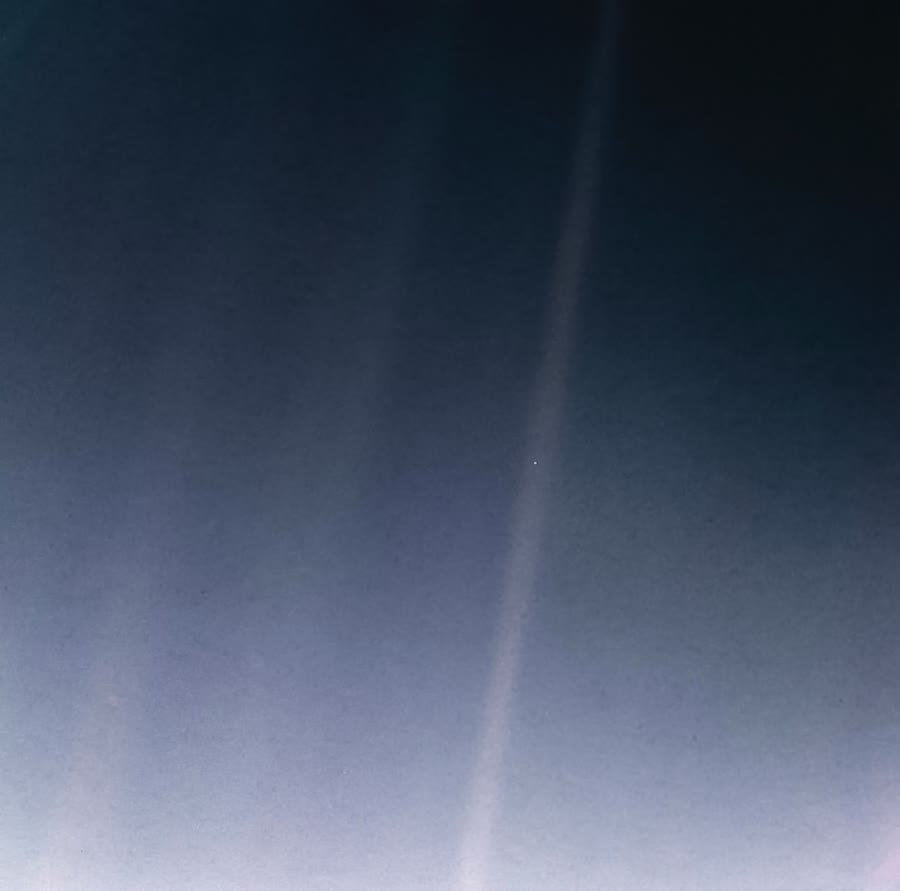
\includegraphics[width=\linewidth]{images/book1/g6-pale-blue-dot.jpg}};
  \draw[yellow!80!orange, thick] ($(img.south west)!0.594!(img.south east) + (0,{0.476*\linewidth})$) circle (6pt);
\end{tikzpicture}\\[2pt]
{\footnotesize A Terra (no círculo) vista pela Voyager~1, 1990. (Imagem:
NASA/JPL-Caltech, domínio público.)}
% ledger: nasa:pale-blue-dot
\end{minipage}
\end{history}

\section{Exercícios}

\begin{exercise}[$\star$]\label{exo:g6:earth-a-planet:1}
Liste os oito planetas do Sistema Solar em ordem, do mais próximo do Sol
ao mais distante. Sublinhe os \omterm{def:g6:earth-a-planet:planet-types}{planetas rochosos}.
\end{exercise}

\begin{exercise}[$\star$]\label{exo:g6:earth-a-planet:2}
Copie e complete: ``Um \omterm{def:g6:earth-a-planet:planet-types}{planeta rochoso} é pequeno e \ldots, com uma
superfície \ldots{} Um \omterm{def:g6:earth-a-planet:planet-types}{planeta gigante} é muito grande, de baixa \ldots,
feito sobretudo de \ldots{} e de \ldots{}''
\end{exercise}

\begin{exercise}[$\star$]\label{exo:g6:earth-a-planet:3}
Usando a tabela deste capítulo, qual planeta tem o diâmetro mais próximo do
da Terra? Qual é o maior planeta? Qual é o menor?
\end{exercise}

\begin{exercise}[$\star$]\label{exo:g6:earth-a-planet:4}
Verdadeiro ou falso? Corrija as frases falsas.
(a) Vênus é coberto de \omterm{def:g2:water-on-earth:ocean}{oceanos}.
(b) Marte é mais frio que a Terra.
(c) Os \omterm{def:g6:earth-a-planet:planet-types}{planetas gigantes} são os quatro planetas mais próximos do Sol.
(d) Saturno é menos denso que a água.
\end{exercise}

\begin{exercise}[$\star\star$]\label{exo:g6:earth-a-planet:5}
O diâmetro de Mercúrio é de 4\,879~km, e o diâmetro da Terra, de
12\,756~km. Calcule o diâmetro de Mercúrio como porcentagem do da Terra,
arredondado para o número inteiro mais próximo.
% ledger: planet:Mercury.diameter, planet:Earth.diameter (planets.py: 38.2 %)
\end{exercise}

\begin{exercise}[$\star\star$]\label{exo:g6:earth-a-planet:6}
Quantas Terras, lado a lado, caberiam no diâmetro de Saturno
(120\,536~km)? Arredonde para o número inteiro mais próximo. Saturno é um
\omterm{def:g6:earth-a-planet:planet-types}{planeta rochoso} ou um \omterm{def:g6:earth-a-planet:planet-types}{planeta gigante}?
% ledger: planet:Saturn.diameter, planet:Earth.diameter
\end{exercise}

\begin{exercise}[$\star\star$]\label{exo:g6:earth-a-planet:7}
Os astrônomos encontraram planetas em volta de outras estrelas. O
planeta~A tem uma densidade de 1.1~grama por centímetro cúbico e é 9~vezes
mais largo que a Terra. O planeta~B tem uma densidade de 5.0~gramas por
centímetro cúbico e é um pouco menor que a Terra. Qual deles é um \omterm{def:g6:earth-a-planet:planet-types}{planeta
rochoso}, e qual é um \omterm{def:g6:earth-a-planet:planet-types}{planeta gigante}? Explique.
\end{exercise}

\begin{exercise}[$\star\star$]\label{exo:g6:earth-a-planet:8}
Usando o gráfico das temperaturas dos planetas: (a) quantos graus Vênus é
mais quente que a Terra? (b) Quantos graus Marte é mais frio que a Terra?
% ledger: planet:Venus.Tmean, planet:Earth.Tmean, planet:Mars.Tmean
\end{exercise}

\begin{exercise}[$\star\star$]\label{exo:g6:earth-a-planet:9}
Mercúrio é o planeta mais próximo do Sol, mas Vênus é o mais quente.
Explique por quê.
\end{exercise}

\begin{exercise}[$\star\star$]\label{exo:g6:earth-a-planet:10}
A Terra fica a 150~milhões de quilômetros do Sol, e Marte a 228~milhões de
quilômetros. Quantos milhões de quilômetros Marte fica mais longe do Sol?
Em que porcentagem a distância de Marte é maior que a da Terra (arredonde
para o número inteiro mais próximo)?
% ledger: planet:Earth.dist, planet:Mars.dist
\end{exercise}

\begin{exercise}[$\star\star\star$]\label{exo:g6:earth-a-planet:11}
Um amigo diz: ``Marte sempre foi um \omterm{def:g5:weather-and-climate:desert}{deserto} seco; nunca houve água ali.''
Usando este capítulo, responda a ele: o que Marte tinha há bilhões de anos,
onde está a sua água hoje, e por que a água líquida não consegue durar na
sua superfície agora?
\end{exercise}

\begin{exercise}[$\star\star\star$]\label{exo:g6:earth-a-planet:12}
Vênus às vezes é chamado de gêmeo da Terra. O seu diâmetro é 95~\% do da
Terra, e a atração da gravidade na sua superfície vale 8.9 numa escala em
que a da Terra vale 9.8. (a) Calcule a atração da gravidade de Vênus como
porcentagem da da Terra,
arredondada para o número inteiro mais próximo. (b) Dê duas maneiras pelas
quais Vênus parece um gêmeo da Terra, e duas maneiras pelas quais não
parece.
% ledger: planet:Venus.gravity, planet:Earth.gravity, planet:Venus.diameter
\end{exercise}

\section{Problema: Cartões-postais de três planetas}

\begin{problem}[{Problema de fim de semana --- três cartões-postais do
espaço, e a força com que o ar de Vênus pressiona o seu chão}]
\label{pb:g6:earth-a-planet:1}
% ledger: planet:Venus.dist, planet:Venus.diameter, planet:Venus.density, planet:Venus.Tmean, planet:Venus.psurf, planet:Earth.dist, planet:Earth.diameter, planet:Earth.density, planet:Earth.Tmean, planet:Earth.psurf, planet:Mars.dist, planet:Mars.diameter, planet:Mars.density, planet:Mars.Tmean, planet:Mars.psurf, nasa:venus-clouds, nasa:mars-water
Três sondas robóticas mandam cada uma um cartão-postal para casa, com
alguns números escritos no verso.

\begin{center}
\small
\begin{tabular}{>{\raggedright\arraybackslash}p{0.29\linewidth}>{\raggedright\arraybackslash}p{0.29\linewidth}>{\raggedright\arraybackslash}p{0.29\linewidth}}
\hline
\textbf{De Vênus} & \textbf{Da Terra} & \textbf{De Marte}\\
\hline
Distância do Sol: 108~milhões~de~km. & Distância do Sol:
150~milhões~de~km. & Distância do Sol: 228~milhões~de~km.\\
Diâmetro: 12\,104~km. & Diâmetro: 12\,756~km. & Diâmetro: 6\,792~km.\\
Densidade: 5.2~g/cm$^3$. & Densidade: 5.5~g/cm$^3$. & Densidade: 3.9~g/cm$^3$.\\
Temperatura média: 464~$^\circ$C. & Temperatura média: 15~$^\circ$C. &
Temperatura média: $-65$~$^\circ$C.\\
O ar pressiona o chão com 92~bar. \omterm{def:g4:clouds-rain-snow:cloud}{Nuvens} espessas de ácido. &
O ar pressiona o chão com 1~bar. \omterm{def:g2:water-on-earth:ocean}{Oceanos} e \omterm{def:g4:clouds-rain-snow:cloud}{nuvens}. &
O ar pressiona o chão com 0.01~bar. Gelo nos \omterm{def:g3:continents-and-oceans:poles}{polos}.\\
\hline
\end{tabular}
\end{center}

\medskip
\noindent\textbf{Parte I --- Os planetas comparados.}
\begin{enumerate}
  \item Coloque os três planetas em ordem de distância do Sol.
  \item Quantos milhões de quilômetros Vênus fica mais perto do Sol que a
        Terra? Quantos milhões de quilômetros Marte fica mais longe?
  \item Calcule o diâmetro de Marte como porcentagem do da Terra,
        arredondado para o número inteiro mais próximo. Marte tem cerca de
        um quarto, da metade ou de três quartos da largura da Terra?
  \item Os três planetas são \omterm{def:g6:earth-a-planet:planet-types}{planetas rochosos} ou \omterm{def:g6:earth-a-planet:planet-types}{planetas gigantes}? Que
        números dos cartões-postais mostram isso?
\end{enumerate}

\medskip
\noindent\textbf{Parte II --- O ar.}
\begin{enumerate}[resume]
  \item Em que planeta o ar é mais espesso? Em qual ele é mais ralo?
  \item Quantas vezes menos o ar de Marte pressiona o seu chão do que o ar
        da Terra pressiona o nosso?
  \item Vênus fica mais perto do Sol que a Terra, mas isso, sozinho, não
        explica uma temperatura de 464~$^\circ$C. O que o ar de Vênus faz
        com o calor do Sol?
  \item Quantas vezes mais forte do que na Terra o ar pressiona o chão de
        Vênus? Por que uma sonda que pousa em Vênus precisa ter paredes muito resistentes?
\end{enumerate}

\medskip
\noindent\textbf{Parte III --- A água e a vida.}
\begin{enumerate}[resume]
  \item Na superfície da Terra, a água congela a 0~$^\circ$C e ferve a
        100~$^\circ$C. Usando as temperaturas médias, explique por que a
        água é líquida na Terra.
  \item O que aconteceria com um copo de água colocado no chão de Vênus?
        E no chão de Marte?
  \item Marte tinha \omterm{def:g1:landscapes-around-us:water}{rios} e \omterm{def:g1:landscapes-around-us:water}{lagos} há bilhões de anos. O que isso nos diz
        sobre o \omterm{def:g5:weather-and-climate:climate}{clima} de Marte há muito tempo, comparado com o de hoje?
  \item Escreva o verso do cartão-postal da Terra: em algumas frases, dê
        quatro motivos pelos quais a vida é possível na Terra.
\end{enumerate}
\end{problem}
